\section{Integer Linear Programming}
\label{sec:co_intro}
\label{chap:chapter_1.1_integer_linear_programming}

This section introduces the integer linear programming framework used in the main contributions of this thesis. We focus mainly on binary integer linear programs (BILPs), in which decision variables take values in $\{0,1\}$ and feasibility is determined by a system of linear constraints. This setting is general enough to encode many classical combinatorial optimization problems, while also exposing the central difficulty studied in this thesis: predicting or constructing binary assignments whose variables are strongly coupled by feasibility constraints. We first define the ILP formalism, then briefly review classical solver components, and finally introduce the graph representations and benchmark problems used in later chapters.

\subsection{Combinatorial optimization and ILP formulations}

Combinatorial optimization (CO) concerns optimization problems whose feasible solutions are discrete objects, such as subsets, paths, matchings, or assignments. Many such problems can be formulated as integer linear programs, which makes ILPs a convenient common language for both classical optimization algorithms and learning-based methods. In this thesis, we focus on binary ILP formulations that explicitly expose variables and constraints, since this structure can be represented as a graph and used as input to neural and graphical-model methods.

\subsection{Problem definition}
The \emph{canonical form} of an ILP is given as
\begin{equation}
    \label{equ:ilp_canonical_form}
    (P) \Leftrightarrow \left\{
    \begin{aligned}
        \max \quad & c^\top x \\
        \text{s.t.} \quad & Ax \leq b, \\
        & x \in \mathcal{X}
    \end{aligned} \right. ,
    % \begin{array}{ll}
    %     \max & c^T x \\
    %     \text{s.t.}              & A x \leq b \\
    %                              & x \in \mathcal{X}
    % \end{array}
\end{equation}
where $x\in \mathcal{X} \subseteq \Z^n$ denotes the vector of decision variables, $c\in\R^n$ is the objective coefficient vector, and $A\in\R^{m\times n}$ and $b\in\R^m$ define the linear constraints. We write $A_j$ for the $j$-th row of $A$, so that the $j$-th constraint is $A_jx \leq b_j$. 

Binary integer linear programs (BILPs), which are the main focus of this thesis, are problems for which $\mathcal{X}=\{0,1\}^n$. An assignment $x$ is called \emph{feasible} if it satisfies both the domain restrictions and the linear constraints; the feasible set is therefore $\FEASIBLESET := \{x\in\mathcal{X} : Ax \leq b\}$.

A formulation is said to be \emph{compact} if the number of variables and constraints is polynomial in the size of the input~\cite{yannakakis_expressing_1988,carr_compact_2000}. This assumption is important for the methods developed in this thesis, since the variable-constraint graph must be represented explicitly. We therefore focus mainly on problems that admit compact BILP formulations. Compactness, however, does not imply that every constraint is small: a compact formulation may still contain constraints involving many variables. This distinction will become important later when we represent constraints through graphical-model structures.

\subsubsection{LP relaxations and solver-state quantities}
Given a BILP with feasible set $\mathcal{X}=\{0,1\}^n$, its linear programming relaxation is obtained by replacing the integrality constraints with continuous bounds:
\begin{equation}
(P_{\mathrm{LP}}) \Leftrightarrow \left\{
\begin{aligned}
\max \quad & c^\top x \\
\text{s.t.} \quad & Ax \leq b, \\
& 0 \leq x \leq 1 .
\end{aligned} \right. .
\end{equation}
The resulting LP provides a continuous approximation of the original integer problem. A point is LP-feasible if it satisfies the linear constraints and the relaxed bounds; it is integer-feasible if it also satisfies the original integrality restrictions. Thus, an LP-feasible solution may be fractional, meaning that some variables satisfy $0<x_i^{\mathrm{LP}}<1$.

LP relaxations provide both bounds for exact solvers and useful information for heuristics and learning models. For a constraint $A_jx\leq b_j$, the slack at an LP solution $x^{\mathrm{LP}}$ is
\begin{equation*}
s_j = b_j - A_jx^{\mathrm{LP}}.
\end{equation*}
A constraint is active, or tight, when $s_j=0$. LP solvers also return dual values associated with constraints, which can be interpreted as sensitivities of the LP objective to changes in the right-hand side, and reduced costs associated with variables, which indicate how variable movements would affect the LP objective around the current optimum.

When the relaxation is solved by the simplex method, the solution is represented by a basis. The corresponding basis status of a variable or constraint records whether it is basic or nonbasic, and, if nonbasic, which bound is active. These quantities are often exposed by MILP solvers and will later be used as optimization-aware features in the variable-constraint graph representation.


\subsection{Solving ILPs}

ILPs can be approached either with algorithms tailored to a specific combinatorial problem or with general-purpose optimization methods. Specialized algorithms can be highly efficient when they exploit additional structure, but they do not provide a uniform framework for arbitrary ILP formulations. In contrast, general-purpose ILP solvers operate directly on the algebraic formulation. This thesis largely follows the latter perspective: the methods developed later take a BILP formulation as input, while using its constraint structure to build graph-based learning and inference models. We therefore briefly review the main solver components that motivate learning-augmented ILP methods.

\subsubsection{Exact approaches}
The most straightforward but impractical approach is exhaustive enumeration of all candidate solutions. More sophisticated exact algorithms exploit structure to prune the search space.

\paragraph{Branch-and-Bound} The Branch-and-Bound (B\&B) method~\cite{land_automatic_1960,dakin_tree-search_1965} explores the solution space through a search tree. At each node, the problem is restricted by branching on a decision variable, yielding subproblems that can be pruned using bounds, infeasibility, or integrality. Figure~\ref{fig:branch_and_bound_tree} illustrates this search-tree structure.

Although B\&B is exact, its worst-case complexity remains exponential, and its practical performance depends heavily on choices such as variable selection, node selection, branching direction, and primal heuristics. These choices provide natural points of intervention for learning-augmented solvers, as reviewed in Chapter~\ref{chap:chapter_2_related_work}. Table~\ref{tab:branch_and_bound_strategies} summarizes these decision points, many of which have been targeted by learning-based methods. Classical examples include strong branching, pseudo-cost and reliability branching, feasibility-pump heuristics, RINS, and local branching~\cite{achterberg_branching_2005,benichou_experiments_1971,fischetti_feasibility_2005,danna_exploring_2005,fischetti_local_2003}.

% \begin{figure}[h!]
% \centering
% \begin{forest}
% for tree={
%     draw,
%     rounded corners,
%     align=center,
%     minimum width=2.2cm,
%     minimum height=1cm,
%     inner sep=2pt,
%     font=\small
% },
% good/.style={fill=green!20},
% bad/.style={fill=red!20},
% neutral/.style={fill=blue!10}
% [P$_0$\\(root)\\{\color{blue}select $x_1$}, neutral
%     [P$_1$\\{\color{blue}$x_1 \le 0$}, good,
%         edge label={node[midway,above,font=\scriptsize]{branch}}
%     ]
%     [P$_2$\\{\color{blue}$x_1 \ge 1$}\\{\color{blue}select $x_2$}, neutral,
%         edge label={node[midway,above,font=\scriptsize]{branch}}
%         [P$_5$\\{\color{blue}$x_2 \le 0$}, bad,
%             edge label={node[midway,above,font=\scriptsize]{prune}}
%         ]
%         [P$_6$\\{\color{blue}$x_2 \ge 1$}, good,
%             edge label={node[midway,above,font=\scriptsize]{feasible}}
%         ]
%     ]
% ]
% \end{forest}
% \caption{Illustration of Branch-and-Bound showing variable selection, branching, and bounding/pruning.}
% \label{fig:branch_and_bound_tree}
% \end{figure}


\begin{figure}[htbp]
\centering

\definecolor{bbActive}{RGB}{225,225,248}
\definecolor{bbFeasible}{RGB}{210,245,210}
\definecolor{bbPruned}{RGB}{255,215,215}
\definecolor{bbBlue}{RGB}{40,80,200}

\tikzset{
    branchlabel/.style={
        midway,
        fill=white,
        inner sep=1pt,
        font=\scriptsize,
        text=black!75
    }
}

\begin{forest}
for tree={
    draw=black!75,
    rounded corners=3pt,
    line width=0.45pt,
    align=center,
    font=\small,
    inner sep=3pt,
    minimum width=2.1cm,
    minimum height=0.85cm,
    edge={-latex, line width=0.45pt, draw=black!70},
    l sep=9mm,
    s sep=10mm,
},
active/.style={fill=bbActive},
feasible/.style={fill=bbFeasible},
pruned/.style={fill=bbPruned}
[
    {$P_0$\\[-1pt]\footnotesize root\\[-1pt]\textcolor{bbBlue}{select $x_1$}},
    active
    [
        {$P_1$\\[-1pt]\textcolor{bbBlue}{$x_1 \le 0$}},
        feasible,
        edge label={node[branchlabel, above left]{branch}}
    ]
    [
        {$P_2$\\[-1pt]\textcolor{bbBlue}{$x_1 \ge 1$}\\[-1pt]\textcolor{bbBlue}{select $x_2$}},
        active,
        edge label={node[branchlabel, above right]{branch}}
        [
            {$P_5$\\[-1pt]\textcolor{bbBlue}{$x_2 \le 0$}},
            pruned,
            edge label={node[branchlabel, above left]{prune}}
        ]
        [
            {$P_6$\\[-1pt]\textcolor{bbBlue}{$x_2 \ge 1$}},
            feasible,
            edge label={node[branchlabel, above right]{feasible}}
        ]
    ]
]
\end{forest}

\caption{Illustration of a branch-and-bound search tree. At each branching node, a variable is selected and the current subproblem is split into child subproblems. Nodes can then be pruned by bounding or retained when they yield feasible incumbent solutions.}
\label{fig:branch_and_bound_tree}
\end{figure}

\begin{table}[H]
    \centering
    \small
    \begin{tabular}{p{0.20\linewidth}p{0.35\linewidth}p{0.35\linewidth}}
        \toprule
        \textbf{Decision} & \textbf{Role in B\&B} & \textbf{Representative strategies} \\
        \midrule
        Node selection 
        & Choose which open subproblem to process next. 
        & Best-bound, depth-first, breadth-first, hybrid strategies, diving. \\
        \midrule
        Variable selection 
        & Choose the variable used to split the current relaxation. 
        & Most-fractional, strong branching, pseudo-cost, reliability branching, ML-based branching. \\
        \midrule
        Branch direction 
        & Choose which child node to explore first. 
        & Reference-solution direction, pseudo-cost direction, inference direction. \\
        \midrule
        Pruning and filtering 
        & Discard nodes or tighten domains when they cannot improve the incumbent. 
        & Infeasibility, bound dominance, integrality, logical inference, reduced-cost fixing. \\
        \midrule
        Primal heuristics 
        & Construct feasible incumbent solutions during the search. 
        & Diving, feasibility pump, RINS, local branching, randomized or ML-guided repair. \\
        \bottomrule
    \end{tabular}
    \caption{Main decision points in Branch-and-Bound and representative strategies. These components are often heuristic and therefore provide natural targets for learning-based solver augmentation.}
    \label{tab:branch_and_bound_strategies}
\end{table}

\paragraph{Cutting planes and Branch-and-Cut}
Cutting planes strengthen the continuous relaxation of an ILP by adding valid inequalities that remove fractional LP solutions while preserving all integer-feasible solutions~\cite{gomory_outline_1958}. Modern MILP solvers combine this idea with B\&B in a Branch-and-Cut framework~\cite{balas_mixed_1996,cochran_branch_2011}: at each node, the LP relaxation is solved, violated cuts may be added to tighten the relaxation, and branching is applied if the relaxed solution remains fractional. Figure~\ref{fig:cutting_plane} illustrates the geometric role of a cut. As with branching, cut separation, cut selection, and cut scheduling involve heuristic choices that can be targeted by learning-based methods. 

Other exact frameworks, such as Branch-and-Price~\cite{barnhart_branch-and-price_1998,cochran_branchpriceandcut_2011}, combine branching with column generation and are particularly useful for formulations with a very large number of variables. They are not central to the methods developed in this thesis, so we do not discuss them further.



\begin{figure}[htbp]
\centering
\begin{tikzpicture}[
    scale=0.85,
    >=Latex,
    line cap=round,
    line join=round,
    every node/.style={font=\small},
    lattice/.style={circle, fill=black, inner sep=1.15pt},
    feasiblept/.style={circle, fill=black, inner sep=1.55pt},
    lpregion/.style={draw=blue!65!black, fill=blue!8, line width=0.0pt},
    cutregion/.style={draw=red!70!black, fill=red!12, line width=0.0pt},
    constraint/.style={blue!70!black, line width=1.0pt},
    cut/.style={red!75!black, dashed, line width=1.1pt},
    solLP/.style={circle, fill=blue!80!black, inner sep=2pt},
    solIP/.style={circle, fill=green!55!black, inner sep=2pt}
]

% --------------------------------------------------
% Parameters
% --------------------------------------------------
\def\eps{0.20}

% Constraint 1: x_2 <= a_1 x_1 + b_1
\pgfmathsetmacro{\aone}{(-1 - 2*\eps)/4}
\pgfmathsetmacro{\bone}{3 + \eps}

% Constraint 2: x_2 <= a_2 x_1 + b_2,
% written as x_2 <= a_2 (x_1 - (5 + eps))
\pgfmathsetmacro{\atwo}{(-3 + 2*\eps)/2}
\pgfmathsetmacro{\btwo}{-\atwo*(5+\eps)}

% Intersection of the two LP constraints = fractional LP optimum
\pgfmathsetmacro{\xLP}{(\btwo-\bone)/(\aone-\atwo)}
\pgfmathsetmacro{\yLP}{\aone*\xLP+\bone}

% Values used for plotting boundaries
\pgfmathsetmacro{\yA}{\bone}
\pgfmathsetmacro{\yB}{\aone*5+\bone}
\pgfmathsetmacro{\yC}{\atwo*5+\btwo}
\pgfmathsetmacro{\xD}{-\btwo/\atwo}

% A Gomory-like illustrative cut, chosen to remove x^LP
% while preserving the integer points below it.
\pgfmathsetmacro{\acut}{-1}
\pgfmathsetmacro{\bcut}{5}

% Intersections of cut with the two LP edges
\pgfmathsetmacro{\xCutOne}{(\bcut-\bone)/(\aone-\acut)}
\pgfmathsetmacro{\yCutOne}{\acut*\xCutOne+\bcut}

\pgfmathsetmacro{\xCutTwo}{(\btwo-\bcut)/(\acut-\atwo)}
\pgfmathsetmacro{\yCutTwo}{\acut*\xCutTwo+\bcut}

% --------------------------------------------------
% Axes
% --------------------------------------------------
\draw[->, thick] (-0.25,0) -- (5.75,0) node[below right] {$x_1$};
\draw[->, thick] (0,-0.25) -- (0,4.35) node[above left] {$x_2$};

% --------------------------------------------------
% Lattice points
% --------------------------------------------------
\foreach \x in {0,...,5}{
  \foreach \y in {0,...,4}{
    \node[lattice, fill=black!35] at (\x,\y) {};
  }
}

% --------------------------------------------------
% Original LP relaxation
% --------------------------------------------------
\filldraw[lpregion]
  (0,0) --
  (\xD,0) --
  %(5,\yC) --
  (\xLP,\yLP) --
  (0,\yA) --
  cycle;


% --------------------------------------------------
% Region removed by the cut
% --------------------------------------------------
\filldraw[cutregion]
  (\xCutOne,\yCutOne) --
  (\xLP,\yLP) --
  (\xD,0) --
  (5,0) --
  cycle;


% Red hatching inside removed part
\begin{scope}
  \clip
    (\xCutOne,\yCutOne) --
    (\xLP,\yLP) --
    (\xD,0) --
    (5,0) --
    cycle;

  \foreach \s in {-2,-1.75,...,6}{
    \draw[red!65, line width=0.65pt]
      (\s,0) -- ++(3.0,3.0);
  }
\end{scope}
% --------------------------------------------------
% Constraint boundaries
% --------------------------------------------------
\draw[constraint] (0,\yA) -- (\xLP,\yLP);
\draw[constraint] (\xLP,\yLP) -- (5,\yC);

% Optional extension of LP boundary lines
\draw[constraint, opacity=0.6]
  (-0.15,{\aone*(-0.15)+\bone})
  --
  (5.45,{\aone*5.45+\bone});

% Stop the second boundary at x_2=0 to avoid drawing below the axis
\draw[constraint, opacity=0.6]
  (2.65,{\atwo*2.65+\btwo})
  --
  ({-\btwo/\atwo},0);

% --------------------------------------------------
% Cutting plane
% --------------------------------------------------
\draw[cut]
  (1.0,4.0)
  --
  (5,0);

\node[red!75!black, above right] at (1.55,{\acut*1.55+\bcut}) {cut};

% --------------------------------------------------
% Feasible integer points: those satisfying both LP constraints and the cut
% --------------------------------------------------
\foreach \x in {0,...,5}{
  \foreach \y in {0,...,4}{
    \pgfmathtruncatemacro{\ok}{
      ifthenelse(
        \y <= \aone*\x+\bone + 0.001 &&
        \y <= \atwo*\x+\btwo + 0.001 &&
        \y <= \acut*\x+\bcut + 0.001,
        1,0)
    }
    \ifnum\ok=1
      \node[feasiblept] at (\x,\y) {};
    \fi
  }
}

% --------------------------------------------------
% Solutions
% --------------------------------------------------
\node[solLP] at (\xLP,\yLP) {};
\node[blue!80!black, above right] at (\xLP,\yLP) {$x^{\mathrm{LP}}$};

\node[solIP] at (3,2) {};
\node[green!45!black, below left] at (3,2) {$x^{\mathrm{IP}}$};

% --------------------------------------------------
% Small label for feasible region
% --------------------------------------------------
%\node[blue!65!black] at (1.25,1.35) {$P_{\mathrm{LP}}$};

\end{tikzpicture}
\caption{Illustration of a cutting plane. The blue shaded region represents the LP relaxation, whose optimum $x^{\mathrm{LP}}$ is attained at a fractional vertex. The dashed red inequality cuts off this fractional solution while preserving the integer-feasible points, including $x^{\mathrm{IP}}$.}
\label{fig:cutting_plane}
\end{figure}

\subsubsection{Primal heuristics and solution construction}

Because exact ILP solving can be computationally expensive, modern solvers rely heavily on primal heuristics to quickly construct feasible incumbent solutions. Examples include diving heuristics, rounding and repair procedures such as the feasibility pump~\cite{fischetti_feasibility_2005}, and neighborhood-based methods such as RINS~\cite{danna_exploring_2005} and VNS~\cite{mladenovic_variable_1997,hansen_variable_2008}. These methods are relevant to this thesis because they highlight a central difficulty: a useful prediction is not merely a vector of independent variable scores, but a coherent assignment that satisfies the constraints. Later chapters address this difficulty by using MRF inference and denoising-based decoding to produce more structured solution predictions.

\paragraph{Diving and tree traversal}
Diving heuristics follow a single branch of the B\&B tree downward, repeatedly selecting promising child nodes until a leaf or infeasible relaxation is reached. This differs from complete traversal strategies such as depth-first search and breadth-first search, which systematically backtrack to explore the tree. Figure~\ref{fig:diving_dfs_bfs} illustrates these different traversal patterns. Diving is particularly relevant in this thesis because several decoding procedures can be interpreted as learned or inference-guided forms of sequential solution construction.

\begin{figure}[H]
    \centering

    %--------------------- DIVING ---------------------%
    \begin{subfigure}{0.32\textwidth}
        \centering
        \begin{tikzpicture}[
            scale=1.0,
            base/.style={circle,draw=gray!60,fill=white,inner sep=1pt,minimum size=5mm},
            treeedge/.style={draw=gray!40},
            feasible/.style={fill=green!30,draw=green!60!black},
            infeasible/.style={fill=red!20,draw=red!70!black,dashed},
            pathDiving/.style={very thick,->,>=Stealth,blue},
        ]
            %--- Nodes (same layout for all subfigures) ---%
            \node[base,infeasible] (r)  at (0,0) {};
            \node[base,infeasible] (a)  at (-1.5,-1.5) {};
            \node[base,infeasible] (b)  at ( 1.5,-1.5) {};
            \node[base,infeasible] (a1) at (-2.3,-3) {};
            \node[base,feasible] (a2) at (-0.7,-3) {};
            \node[base,feasible] (b1) at ( 0.7,-3) {};
            \node[base,infeasible] (b2) at ( 2.3,-3) {};

            %--- Tree edges (faint) ---%
            \draw[treeedge] (r) -- (a);
            \draw[treeedge] (r) -- (b);
            \draw[treeedge] (a) -- (a1);
            \draw[treeedge] (a) -- (a2);
            \draw[treeedge] (b) -- (b1);
            \draw[treeedge] (b) -- (b2);

            %--- Diving path: root -> left child -> left grandchild ---%
            \draw[pathDiving] (r) to[bend left=5] (a);
            \draw[pathDiving] (a) to[bend left=5] (a1);

        \end{tikzpicture}
        \caption{Diving: single guided root-to-leaf path}
        \label{fig:diving_path}
    \end{subfigure}
    \hfill
    %--------------------- DFS ---------------------%
    \begin{subfigure}{0.32\textwidth}
        \centering
        \begin{tikzpicture}[
            scale=1.0,
            base/.style={circle,draw=gray!60,fill=white,inner sep=1pt,minimum size=5mm},
            feasible/.style={fill=green!30,draw=green!60!black},
            infeasible/.style={fill=red!20,draw=red!70!black,dashed},
            treeedge/.style={draw=gray!40},
            pathDFS/.style={very thick,->,>=Stealth,red},
        ]
            %--- Nodes ---%
            \node[base,infeasible] (r)  at (0,0) {};
            \node[base,infeasible] (a)  at (-1.5,-1.5) {};
            \node[base,infeasible] (b)  at ( 1.5,-1.5) {};
            \node[base,infeasible] (a1) at (-2.3,-3) {};
            \node[base,feasible] (a2) at (-0.7,-3) {};
            \node[base,feasible] (b1) at ( 0.7,-3) {};
            \node[base,infeasible] (b2) at ( 2.3,-3) {};

            %--- Tree edges (faint) ---%
            \draw[treeedge] (r) -- (a);
            \draw[treeedge] (r) -- (b);
            \draw[treeedge] (a) -- (a1);
            \draw[treeedge] (a) -- (a2);
            \draw[treeedge] (b) -- (b1);
            \draw[treeedge] (b) -- (b2);

            %--- DFS path (with backtracking, using bent arrows) ---%
            % r -> a -> a1
            \draw[pathDFS] (r)  to[bend left=5] (a);
            \draw[pathDFS] (a)  to[bend left=5] (a1);
            % backtrack a1 -> a
            %\draw[pathDFS] (a1) to[bend left=40] (a);
            % a -> a2
            \draw[pathDFS] (a1)  to[bend left=5] (a2);


        \end{tikzpicture}
        \caption{Depth-first search with backtracking}
        \label{fig:dfs_path}
    \end{subfigure}
    \hfill
    %--------------------- BFS ---------------------%
    \begin{subfigure}{0.32\textwidth}
        \centering
        \begin{tikzpicture}[
            scale=1.0,
            base/.style={circle,draw=gray!60,fill=white,inner sep=1pt,minimum size=5mm},
            feasible/.style={fill=green!30,draw=green!60!black},
            infeasible/.style={fill=red!20,draw=red!70!black,dashed},
            treeedge/.style={draw=gray!40},
            pathBFS/.style={very thick,->,>=Stealth,green!60!black},
        ]
            %--- Nodes ---%
            \node[base,infeasible] (r)  at (0,0) {};
            \node[base,infeasible] (a)  at (-1.5,-1.5) {};
            \node[base,infeasible] (b)  at ( 1.5,-1.5) {};
            \node[base,infeasible] (a1) at (-2.3,-3) {};
            \node[base,feasible] (a2) at (-0.7,-3) {};
            \node[base,feasible] (b1) at ( 0.7,-3) {};
            \node[base,infeasible] (b2) at ( 2.3,-3) {};

            %--- Tree edges (faint) ---%
            \draw[treeedge] (r) -- (a);
            \draw[treeedge] (r) -- (b);
            \draw[treeedge] (a) -- (a1);
            \draw[treeedge] (a) -- (a2);
            \draw[treeedge] (b) -- (b1);
            \draw[treeedge] (b) -- (b2);

            %--- BFS path (level by level, with bent backtracking to root/parent) ---%
            % Level 0 -> Level 1
            %\draw[pathBFS] (r)  to[bend left=5] (a);
            %\draw[pathBFS] (a)  to[bend left=40] (r);
            %\draw[pathBFS] (r)  to[bend left=5] (b);
            %\draw[pathBFS] (b)  to[bend left=40] (r);
            % Level 1 -> Level 2
            %\draw[pathBFS] (r)  to[bend left=20] (a1);
            %\draw[pathBFS] (a1) to[bend left=40] (r);
            %\draw[pathBFS] (r)  to[bend left=0]  (a2);

            \draw[pathBFS] (r) to[bend left=5] (a);
            \draw[pathBFS] (a) to (b);
            \draw[pathBFS] (b) to (a1);
            \draw[pathBFS] (a1) to (a2);

            

        \end{tikzpicture}
        \caption{Breadth-first search visiting nodes by level}
        \label{fig:bfs_path}
    \end{subfigure}

    \caption{Schematic comparison of Diving (blue), depth-first search (red), and breadth-first search (green) traversal patterns on the same search tree. Faint gray edges show the full tree; colored arrows indicate the order in which nodes are visited.}
    \label{fig:diving_dfs_bfs}
\end{figure}

\paragraph{Rounding and feasibility pump}
Another class of primal heuristics attempts to construct an integer solution that is close to a fractional solution of the LP relaxation. Simple rounding strategies directly round fractional variables to nearby integer values and may apply repair procedures to restore feasibility. However, independently rounding the variables of an LP solution can easily produce an integer point that violates the original constraints.

The Feasibility Pump~\cite{fischetti_feasibility_2005} addresses this issue through an alternating projection scheme. Starting from a fractional LP-feasible solution $x^{\mathrm{LP}}$, the method first computes an integer point $x^I$ by rounding the integer-constrained components. If $x^I$ satisfies the original constraints, the procedure terminates with an integer-feasible solution. Otherwise, $x^I$ is projected back onto the LP relaxation by solving a continuous proximity optimization problem, yielding a new LP-feasible point $x^{\mathrm{proj}}$. The method then repeats by rounding $x^{\mathrm{proj}}$ to a new integer point. If the algorithm detects cycling or stalling, the current integer point may be perturbed before the projection step is performed.

\paragraph{Neighborhood-based improvement heuristics}
Neighborhood-based improvement heuristics attempt to refine a current incumbent integer solution by exploring a restricted subset of the feasible region. Two representative methods are \emph{Relaxation Induced Neighborhood Search} (RINS)~\cite{danna_exploring_2005} and \emph{Variable Neighborhood Search} (VNS)~\cite{mladenovic_variable_1997,hansen_variable_2008}.

Let $\operatorname{round}(x^{\mathrm{LP}}_i)$ denote a nearest integer value to $x^{\mathrm{LP}}$. RINS fixes the variables whose incumbent value agrees with the rounded LP-relaxation value. It then fixes this agreement set and solves a reduced MILP, searching within a neighborhood containing all feasible solutions consistent with the common components of $x^{\mathrm{inc}}$ and $x^{\mathrm{LP}}$.

VNS, in contrast, explores a sequence of expanding neighborhoods around the incumbent. For binary or integer variables, a typical choice is a $k$-flip neighborhood. A generic VNS iteration consists of: (i) a \emph{shaking} step that selects a point at distance $k$ from the incumbent, (ii) a local improvement phase, and (iii) an update rule that either accepts the improved solution and resets the neighborhood size, or increases it. This systematic enlargement helps escape local minima while intensifying search around promising regions.

Both RINS and VNS follow the large-neighborhood search philosophy: they construct a restricted subproblem around the incumbent, attempt to improve it, and update the incumbent whenever a better solution is found.

\subsection{Variable-constraint bipartite representation}
\label{sec:vcg_definition}

Representing an ILP as a graph is central to several methods studied in this thesis. A graph representation of mixed-integer linear optimization problems was notably used by Gasse et al.~\cite{gasse_exact_2019} through the \emph{variable-constraint bipartite graph}.

\begin{definition}[Variable-constraint bipartite representation of an ILP]
    Given an ILP instance $(P)$ in canonical form~\eqref{equ:ilp_canonical_form}, its \emph{variable-constraint bipartite representation} is the bipartite graph $\VCGFULL$, where $\VCGV$ contains one node for each decision variable and $\VCGC$ contains one node for each constraint, i.e., each row $A_j x \leq b_j$. The edge set $\VCGE \subseteq \VCGV \times \VCGC$ is defined by
    \begin{equation*}
        (i,j)\in \VCGE
        \quad \Longleftrightarrow \quad
        A_{ji} \neq 0,
    \end{equation*}
    that is, a variable node is connected to a constraint node whenever the corresponding variable appears with nonzero coefficient in that constraint.
\end{definition}

It is important to distinguish this representation from the factor graphs introduced later. The variable-constraint graph is an input representation of the ILP, typically used by GNN encoders. A factor graph, by contrast, will later be used to define the factorization of a probability distribution or energy model over solution variables. In many of our models the two graphs are closely related, because constraints in the ILP will later give rise to factors in the MRF, but they play different roles.

% \begin{figure}[H]
%     \centering

%     % ---------------- LEFT PANEL ----------------
%     \begin{minipage}[c]{0.42\textwidth}
%     \centering
%     \begin{tikzpicture}
%         \node[
%             draw,
%             rounded corners=4pt,
%             align=left,
%             inner sep=10pt,
%             text width=0.9\linewidth,
%             font=\small
%         ] {
%         \textbf{ILP}\\[0.4em]
%         $\max \quad x_1 + x_2 + x_3$\\[0.4em]
%         \text{s.t.}\quad $x_1 + x_2 \leq 1,$\\
%         \hspace*{2.35em}$x_2 + x_3 \leq 1,$\\
%         \hspace*{2.35em}$x_1 + x_2 + x_3 \leq 3,$\\[0.3em]
%         \hspace*{2.35em}$x_i \in \{0,1\}, \quad i=1,2,3.$
%         };
%     \end{tikzpicture}
%     \end{minipage}
%     \hspace{2em}
%     % ---------------- RIGHT PANEL ----------------
%     \begin{minipage}[c]{0.48\textwidth}
%     \centering
%     \begin{tikzpicture}[
%         x=1.3cm, y=1.2cm,
%         var/.style={
%             circle,
%             draw,
%             thick,
%             minimum size=8mm,
%             inner sep=0pt,
%             fill=blue!15
%         },
%         con/.style={
%             rectangle,
%             draw,
%             thick,
%             minimum width=8mm,
%             minimum height=8mm,
%             inner sep=1pt,
%             fill=orange!20
%         },
%         edge/.style={draw, thick}
%     ]

%     % Variable nodes
%     \node[var] (x1) at (0,2) {$x_1$};
%     \node[var] (x2) at (0,1) {$x_2$};
%     \node[var] (x3) at (0,0) {$x_3$};

%     % Constraint nodes
%     \node[con] (c1) at (3,2) {$c_1$};
%     \node[con] (c2) at (3,1) {$c_2$};
%     \node[con] (c3) at (3,0) {$c_3$};

%     % Edges
%     \draw[edge] (x1) -- (c1);
%     \draw[edge] (x2) -- (c1);

%     \draw[edge] (x2) -- (c2);
%     \draw[edge] (x3) -- (c2);

%     \draw[edge] (x1) -- (c3);
%     \draw[edge] (x2) -- (c3);
%     \draw[edge] (x3) -- (c3);

%     % Optional labels
%     \node[anchor=west, font=\scriptsize] at (3.35,2) {$x_1+x_2\leq 1$};
%     \node[anchor=west, font=\scriptsize] at (3.35,1) {$x_2+x_3\leq 1$};
%     \node[anchor=west, font=\scriptsize] at (3.35,0) {$x_1+x_2+x_3\leq 3$};

%     \end{tikzpicture}
%     \end{minipage}

%     \caption{Illustration of an integer linear program and its associated variable-constraint bipartite graph representation. Variable nodes are connected to the constraints in which they appear.}
%     \label{fig:vcg_example}
% \end{figure}

\begin{figure}[H]
    \centering

    % ================= LEFT PANEL =================
    \begin{minipage}[c]{0.44\textwidth}
        \centering
        \begin{tikzpicture}
            \node[
                draw=black!70,
                rounded corners=6pt,
                line width=0.8pt,
                fill=gray!5,
                inner sep=10pt,
                text width=0.9\linewidth,
                align=left
            ] (ilpbox) {%
                {\bfseries Small binary ILP}\\[0.6em]
                $\displaystyle \max \; 6x_1 + 5x_2 + 4x_3$\\[0.6em]
                \text{s.t.}\\[0.2em]
                $\displaystyle 2x_1 + x_2 + x_3 \le 3,$\\[0.3em]
                $\displaystyle x_1 + 2x_2 + x_3 \le 3,$\\[0.3em]
                $\displaystyle x_1,x_2,x_3 \in \{0,1\}.$
            };

            \node[font=\scriptsize, text=black!60, below=4pt of ilpbox.south] {};
        \end{tikzpicture}
    \end{minipage}
    \hspace{2em}
    % ================= RIGHT PANEL =================
    \begin{minipage}[c]{0.48\textwidth}
        \centering
        \begin{tikzpicture}[
            x=1.35cm,
            y=1.25cm,
            var/.style={
                circle,
                draw=blue!60!black,
                fill=blue!12,
                thick,
                minimum size=9mm,
                inner sep=0pt,
                font=\small
            },
            con/.style={
                rounded rectangle,
                draw=orange!70!black,
                fill=orange!18,
                thick,
                minimum width=10mm,
                minimum height=8mm,
                inner sep=2pt,
                font=\small
            },
            ed/.style={
                draw=black!65,
                line width=0.9pt
            },
            lab/.style={
                font=\scriptsize,
                text=black!70,
                align=left
            }
        ]

            % Variables
            \node[var] (x1) at (0,2) {$x_1$};
            \node[var] (x2) at (0,1) {$x_2$};
            \node[var] (x3) at (0,0) {$x_3$};

            % Constraints
            \node[con] (c1) at (3,1.5) {$c_1$};
            \node[con] (c2) at (3,0.5) {$c_2$};

            % Edges for c1: 2x1 + x2 + x3 <= 3
            \draw[ed] (x1) -- (c1);
            \draw[ed] (x2) -- (c1);
            \draw[ed] (x3) -- (c1);

            % Edges for c2: x1 + 2x2 + x3 <= 3
            \draw[ed] (x1) -- (c2);
            \draw[ed] (x2) -- (c2);
            \draw[ed] (x3) -- (c2);

            % Constraint labels
            \node[lab, anchor=west] at (3.45,1.5) {$2x_1 + x_2 + x_3 \le 3$};
            \node[lab, anchor=west] at (3.45,0.5) {$x_1 + 2x_2 + x_3 \le 3$};

            % Small headers
            \node[font=\scriptsize\bfseries, text=blue!60!black] at (0,2.7) {Variables};
            \node[font=\scriptsize\bfseries, text=orange!70!black] at (3,2.7) {Constraints};

        \end{tikzpicture}
    \end{minipage}

    \caption{A small binary integer linear program and its variable-constraint bipartite graph representation. Variable nodes are connected to the constraint nodes in which they appear.}
    \label{fig:vcg_example}
\end{figure}

The graph $\VCGFULL$ can be enriched with node and edge features. Node features may encode quantities associated with variables or constraints, such as objective coefficients, right-hand-side values, slack values, fractional values, dual information, or basis status. Edge features may similarly encode the coefficient $A_{ji}$ associated with variable $i$ in constraint $j$.

This representation offers several advantages. First, it provides a sparse encoding whose structure is independent of the ordering of variables and constraints of the optimization problem structure, making it well suited to graph-based learning architectures. Second, it allows instances of different sizes to be processed within a common framework and to be batched together as disconnected components of a larger graph. Finally, this representation is closely related to the factor graph formalism introduced later in Section~\ref{sec:mrf_intro}, which will be central to our Markov random field models.


\subsection{Representative problems}
We use Maximum Independent Set (MIS) and Set Cover (SC) as representative BILP families. Both are classical NP-hard combinatorial optimization problems~\cite{miller_reducibility_1972}, and together they illustrate two different constraint structures: pairwise exclusion constraints for MIS and potentially high-arity coverage constraints for SC.

\subsubsection{Maximum Independent Set}  
Given an undirected graph $\GFULL$, find the largest subset $S \subseteq \GV$ such that no two vertices in $S$ are adjacent. MIS is equivalent to finding the maximum clique in the complement graph, with applications in network analysis, scheduling, and computational biology. Introducing a binary decision variable $x_i$ for each vertex $i\in\GV$, the standard edge-based BILP formulation is
\begin{align}
    \label{equ:mis_formulation_edges}
    (P_\text{MIS}) \Leftrightarrow \left\{
    \begin{array}{lll}
        \max        & \mathds{1}^T x   & \\
        \text{s.t.} & x_i + x_j \leq 1 & \forall (i,j) \in \GE \\
                    & x \in \{0,1\}^n
    \end{array}
    \right.
\end{align}
Figure~\ref{fig:mis_example} illustrates an independent set and a maximum independent set on a small graph.

\begin{figure}[H]
	\centering
	\input{resources/tikz/chapter_1/co/mis_example}
	\hspace{2em}
	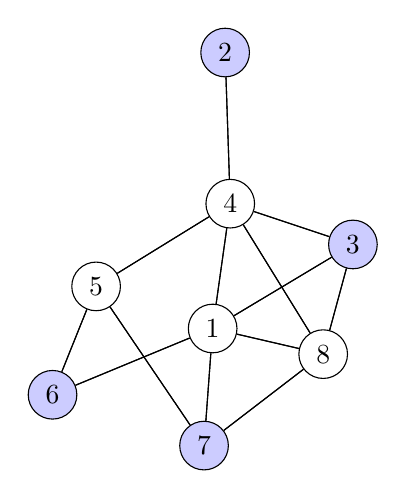
\begin{tikzpicture}[
	every node/.style={draw,circle,fill=white}
	]
	\node  (1) at (0.007009540975573363, -0.5047938530583475)  { 1 };
	\node[fill=blue!20]  (2) at (0.1655944806897962, 3.0)  { 2 };
	\node[fill=blue!20]  (3) at (1.7882499477335903, 0.5624667603559526)  { 3 };
	\node  (4) at (0.2304467971034299, 1.0805731000625989)  { 4 };
	\node  (5) at (-1.473143231371646, 0.02991880959488384)  { 5 };
	\node[fill=blue!20]  (6) at (-2.0265026416974, -1.34637492706497)  { 6 };
	\node[fill=blue!20]  (7) at (-0.10230346491273862, -1.9915902628063684)  { 7 };
	\node  (8) at (1.4106485714793942, -0.8301996270837496)  { 8 };
	\path[draw]  (1) -- (3);
	\path[draw]  (1) -- (4);
	\path[draw]  (1) -- (6);
	\path[draw]  (1) -- (7);
	\path[draw]  (1) -- (8);
	\path[draw]  (2) -- (4);
	\path[draw]  (3) -- (1);
	\path[draw]  (3) -- (4);
	\path[draw]  (3) -- (8);
	\path[draw]  (4) -- (1);
	\path[draw]  (4) -- (2);
	\path[draw]  (4) -- (3);
	\path[draw]  (4) -- (5);
	\path[draw]  (4) -- (8);
	\path[draw]  (5) -- (4);
	\path[draw]  (5) -- (6);
	\path[draw]  (5) -- (7);
	\path[draw]  (6) -- (1);
	\path[draw]  (6) -- (5);
	\path[draw]  (7) -- (1);
	\path[draw]  (7) -- (5);
	\path[draw]  (7) -- (8);
	\path[draw]  (8) -- (1);
	\path[draw]  (8) -- (3);
	\path[draw]  (8) -- (4);
	\path[draw]  (8) -- (7);
\end{tikzpicture}

	\caption{Maximum Independent Set example. The left set is independent, while the right set is a maximum independent set for this graph.}
	\label{fig:mis_example}
\end{figure}

Each constraint $x_i+x_j\leq 1$ prevents adjacent vertices from being selected simultaneously. Together with the binary constraints, these inequalities encode the independent sets of $\G$. Although correct, the edge formulation can have a weak LP relaxation. It can be strengthened using clique inequalities: in any clique $c\subseteq\GV$, at most one vertex can belong to an independent set. Let $\mathcal{C}$ denote a collection of cliques in $\G$; this yields the formulation
\begin{align}
    \label{equ:mis_formulation_cliques}
    (P_\mathrm{MIS}) \Leftrightarrow \left\{
    \begin{array}{lll}
        \max        & \mathds{1}^T x   & \\
        \text{s.t.} & \sum_{i\in c} x_i \leq 1 & \forall c \in \mathcal{C} \\
                    & x \in \{0,1\}^n
    \end{array}
    \right.
\end{align}
The number of cliques can, however, be exponential in $n$, so the full clique formulation is generally not compact. In practice, one may restrict attention to maximal cliques or add violated clique constraints dynamically. This example illustrates a recurring trade-off: stronger formulations may introduce larger or more numerous constraints, which later affects the graphical models built from these constraints.

\subsubsection{Set Cover} 
Given a universe of items $\ITEMS=\{\ITEM_i\}_{i=1}^m$ and a collection of sets $\SCSETS=\{\SCSET_j\}_{j=1}^n$, the objective is to select as few sets as possible while covering every item. We introduce a binary variable $x_j$ for each set $\SCSET_j \in \SCSETS$, and denote by $\SCSETI$ the collection of sets that contain item $\ITEM_i$. The BILP formulation is:
\begin{align}
    \label{equ:sc_formulation}
    (P_\mathrm{SC}) \Leftrightarrow \left\{
    \begin{array}{lll}
        \min        & \mathds{1}^T x   & \\
        \text{s.t.} & \sum_{j:\SCSET_j \in \SCSETI} x_j \geq 1 & \forall 1 \leq i \leq m \\
                    & x \in \{0,1\}^n
    \end{array}
    \right.
\end{align}

Unlike the edge-based MIS formulation, a single SC constraint may involve many variables, since an item can belong to many sets. This makes SC a useful benchmark for feasibility-aware prediction and also foreshadows a scalability issue studied later in the thesis: graphical models built directly from such constraints must handle interactions among many variables at once. Figure~\ref{fig:set_cover_example} illustrates a small SC instance.

\begin{figure}[H]
\centering
\begin{tikzpicture}[scale=1.0]

    % Universe elements
    \node[circle,draw,fill=white,minimum size=7mm] (e1) at (0,0) {1};
    \node[circle,draw,fill=white,minimum size=7mm] (e2) at (2,0) {2};
    \node[circle,draw,fill=white,minimum size=7mm] (e3) at (4,0) {3};
    \node[circle,draw,fill=white,minimum size=7mm] (e4) at (1,-1.8) {4};
    \node[circle,draw,fill=white,minimum size=7mm] (e5) at (3,-1.8) {5};

    % Styles for the sets
    \tikzset{
        setS1/.style={draw=green!60!black,   fill=blue!40,   ellipse, opacity=0.25, inner sep=8pt, line width=2.2pt},
        setS2/.style={draw=red!60!black,    fill=red!50,    ellipse, opacity=0.25, inner sep=8pt},
        setS3/.style={draw=green!60!black, fill=green!50, ellipse, opacity=0.25, inner sep=8pt},
        setS4/.style={draw=green!60!black, fill=orange!70, ellipse, opacity=0.25, inner sep=8pt, line width=2.2pt}
    }

    % Sets as transparent ellipses fitted around the nodes
    \begin{scope}[on background layer]
        % S1 = {1,2,4}
        \node[setS1,fit=(e1)(e2)(e4)] (S1box) {};
        % S2 = {2,3,5}
        \node[setS2,fit=(e2)(e3)] (S2box) {};
        % S3 = {1,4,5}
        \node[setS3,fit=(e4)(e5)] (S3box) {};
        % S4 = {3,4}
        \node[setS4,rotate=-30,fit=(e3)(e5)]     (S4box) {};
    \end{scope}

    % Labels for the sets (placed near ellipse anchors)
    \node[blue!70!black,anchor=south west]  at (S1box.north west) {\scriptsize $S_1=\{1,2,4\}$};
    \node[red!80!black,anchor=south east]   at (S2box.north east) {\scriptsize $S_2=\{2,3\}$};
    \node[green!70!black,anchor=north west] at (S3box.south west) {\scriptsize $S_3=\{4,5\}$};
    \node[orange!80!black,anchor=north east]at (S4box.south east) {\scriptsize $S_4=\{3,5\}$};

\end{tikzpicture}
\caption{Set covering illustration with sets $S_1,\dots,S_4$ covering the universe $U=\{1,2,3,4,5\}$. The minimal set cover is $\{ S_1, S_4 \}$.}
\label{fig:set_cover_example}
\end{figure}


\subsection{Summary: ILPs as structured prediction inputs}

This section introduced BILP formulations, the classical solver context, and the graph representation used to encode ILP structure. The key point for the remainder of the thesis is that feasibility constraints couple the binary decision variables: predicting each variable independently is generally insufficient to obtain a valid solution. The variable-constraint graph provides a natural input representation for learning models, while later sections will show how related graphical structures can represent interactions between solution variables.

The next sections build on this view by introducing neural models for structured prediction and Markov Random Fields for representing and inferring over coupled solution variables. The high-arity constraints that arise in problems such as Set Cover will later motivate approximate graphical parameterizations.